%Version 3.1 December 2024
% See section 11 of the User Manual for version history
%
%%%%%%%%%%%%%%%%%%%%%%%%%%%%%%%%%%%%%%%%%%%%%%%%%%%%%%%%%%%%%%%%%%%%%%
%%                                                                 %%
%% Please do not use \input{...} to include other tex files.       %%
%% Submit your LaTeX manuscript as one .tex document.              %%
%%                                                                 %%
%% All additional figures and files should be attached             %%
%% separately and not embedded in the \TeX\ document itself.       %%
%%                                                                 %%
%%%%%%%%%%%%%%%%%%%%%%%%%%%%%%%%%%%%%%%%%%%%%%%%%%%%%%%%%%%%%%%%%%%%%

%%\documentclass[referee,sn-basic]{sn-jnl}% referee option is meant for double line spacing

%%=======================================================%%
%% to print line numbers in the margin use lineno option %%
%%=======================================================%%

%%\documentclass[lineno,pdflatex,sn-basic]{sn-jnl}% Basic Springer Nature Reference Style/Chemistry Reference Style

%%=========================================================================================%%
%% the documentclass is set to pdflatex as default. You can delete it if not appropriate.  %%
%%=========================================================================================%%

%%\documentclass[sn-basic]{sn-jnl}% Basic Springer Nature Reference Style/Chemistry Reference Style

%%Note: the following reference styles support Namedate and Numbered referencing. By default the style follows the most common style. To switch between the options you can add or remove “Numbered” in the optional parenthesis. 
%%The option is available for: sn-basic.bst, sn-chicago.bst%  
 
%%\documentclass[pdflatex,sn-nature]{sn-jnl}% Style for submissions to Nature Portfolio journals
%%\documentclass[pdflatex,sn-basic]{sn-jnl}% Basic Springer Nature Reference Style/Chemistry Reference Style
\documentclass[pdflatex,sn-mathphys-num]{sn-jnl}% Math and Physical Sciences Numbered Reference Style
%%\documentclass[pdflatex,sn-mathphys-ay]{sn-jnl}% Math and Physical Sciences Author Year Reference Style
%%\documentclass[pdflatex,sn-aps]{sn-jnl}% American Physical Society (APS) Reference Style
%%\documentclass[pdflatex,sn-vancouver-num]{sn-jnl}% Vancouver Numbered Reference Style
%%\documentclass[pdflatex,sn-vancouver-ay]{sn-jnl}% Vancouver Author Year Reference Style
%%\documentclass[pdflatex,sn-apa]{sn-jnl}% APA Reference Style
%%\documentclass[pdflatex,sn-chicago]{sn-jnl}% Chicago-based Humanities Reference Style

%%%% Standard Packages
%%<additional latex packages if required can be included here>

\usepackage{graphicx}%
\usepackage{multirow}%
\usepackage{amsmath,amssymb,amsfonts}%
\usepackage{amsthm}%
\usepackage{mathrsfs}%
\usepackage[title]{appendix}%
\usepackage{xcolor}%
\usepackage{textcomp}%
\usepackage{manyfoot}%
\usepackage{booktabs}%
\usepackage{algorithm}%
\usepackage{algorithmicx}%
\usepackage{algpseudocode}%
\usepackage{listings}%
%%%%

\usepackage{tabularx}
\usepackage{booktabs}
\usepackage{array}
\usepackage{makecell}

%%%%%=============================================================================%%%%
%%%%  Remarks: This template is provided to aid authors with the preparation
%%%%  of original research articles intended for submission to journals published 
%%%%  by Springer Nature. The guidance has been prepared in partnership with 
%%%%  production teams to conform to Springer Nature technical requirements. 
%%%%  Editorial and presentation requirements differ among journal portfolios and 
%%%%  research disciplines. You may find sections in this template are irrelevant 
%%%%  to your work and are empowered to omit any such section if allowed by the 
%%%%  journal you intend to submit to. The submission guidelines and policies 
%%%%  of the journal take precedence. A detailed User Manual is available in the 
%%%%  template package for technical guidance.
%%%%%=============================================================================%%%%

%% as per the requirement new theorem styles can be included as shown below
\theoremstyle{thmstyleone}%
\newtheorem{theorem}{Theorem}%  meant for continuous numbers
%%\newtheorem{theorem}{Theorem}[section]% meant for sectionwise numbers
%% optional argument [theorem] produces theorem numbering sequence instead of independent numbers for Proposition
\newtheorem{proposition}[theorem]{Proposition}% 
%%\newtheorem{proposition}{Proposition}% to get separate numbers for theorem and proposition etc.

\theoremstyle{thmstyletwo}%
\newtheorem{example}{Example}%
\newtheorem{remark}{Remark}%

\theoremstyle{thmstylethree}%
\newtheorem{definition}{Definition}%

\raggedbottom
%%\unnumbered% uncomment this for unnumbered level heads


\newcommand{\TODO}[1]{\textcolor{red}{[TODO: #1]}}
\begin{document}

\title{A Comparative Analysis of Semantic Attributes for Research Software Classification: Evidence from Papers with Code and bio.tools}

%%=============================================================%%
%% GivenName	-> \fnm{Joergen W.}
%% Particle	-> \spfx{van der} -> surname prefix
%% FamilyName	-> \sur{Ploeg}
%% Suffix	-> \sfx{IV}
%% \author*[1,2]{\fnm{Joergen W.} \spfx{van der} \sur{Ploeg} 
%%  \sfx{IV}}\email{iauthor@gmail.com}
%%=============================================================%%

\author*[1,2]{\fnm{First} \sur{Author}}\email{iauthor@gmail.com}

\author[2,3]{\fnm{Second} \sur{Author}}\email{iiauthor@gmail.com}
\equalcont{These authors contributed equally to this work.}

\author[1,2]{\fnm{Third} \sur{Author}}\email{iiiauthor@gmail.com}
\equalcont{These authors contributed equally to this work.}

\affil*[1]{\orgdiv{Department}, \orgname{Organization}, \orgaddress{\street{Street}, \city{City}, \postcode{100190}, \state{State}, \country{Country}}}

\affil[2]{\orgdiv{Department}, \orgname{Organization}, \orgaddress{\street{Street}, \city{City}, \postcode{10587}, \state{State}, \country{Country}}}

\affil[3]{\orgdiv{Department}, \orgname{Organization}, \orgaddress{\street{Street}, \city{City}, \postcode{610101}, \state{State}, \country{Country}}}

%%==================================%%
%% Sample for unstructured abstract %%
%%==================================%%

\abstract{Research Software repositories describe software through heterogeneous metadata schemas, controlled vocabularies, and levels of detail. This heterogeneity limits cross-repository discovery and complicates the use of repository metadata for classification. This paper compares semantic metadata attributes in Papers with Code and bio.tools using a harmonized final dataset of 56,819 labelled Research Software records. We align retained repository fields into a unified semantic framework and quantify metadata coverage, completeness, semantic richness, semantic overlap, and repository-specific availability. We further evaluate how textual metadata attributes support supervised Research Software classification using completed TF--IDF LinearSVC experiments with deterministic train/test splits. The two repositories show no literal overlap between final label vocabularies, but substantial overlap at schema and field-availability levels. Metadata completeness is high in both sources, with mean completeness of 0.8089 for Papers with Code and 0.8192 for bio.tools. In the completed local classification experiments, all available metadata gives the strongest macro-F1 for each evaluated dataset, reaching 0.8671 for Papers with Code single-label records, 0.8782 for Papers with Code multi-label records, 0.4728 for bio.tools single-label records, and 0.6644 for bio.tools multi-label records. The results show that conceptual metadata harmonization can expose shared structure across distinct repository vocabularies, while classification performance remains sensitive to label space, domain, and attribute availability.}


\keywords{Research Software, Metadata, Semantic Attributes, Research Software Classification, Papers with Code, bio.tools, EDAM, TF--IDF}


\maketitle


\section{Introduction}
\label{sec:introduction}

Research Software has become an essential component of contemporary scientific practice. Software supports data acquisition, simulation, analysis, visualization, and reproducibility, and is increasingly treated as a scholarly output in its own right. The FAIR principles and their Research Software extension emphasize that software should be findable, accessible, interoperable, and reusable, and that these goals depend on rich and machine-actionable metadata \cite{Wilkinson2016FAIR,Lamprecht2020FAIRSoftware,Barker2022FAIR4RS,FAIR4RS2022Principles}. Software citation guidance similarly highlights the importance of metadata for attribution and reuse \cite{Smith2016SoftwareCitation}.

Research Software metadata are distributed across heterogeneous repositories. Papers with Code links publications to implementations and organizes artificial-intelligence research through tasks, methods, datasets, and benchmarks. bio.tools describes Life Science software through the biotoolsSchema and EDAM ontology, including topics and operations \cite{Ison2013EDAM,Ison2019BioTools,Ison2021BioToolsSchema}. These resources share the broad goal of improving software discovery, yet they differ in vocabulary, metadata structure, domain, and curation practice. Such differences complicate cross-repository metadata integration and the development of general Research Software classification workflows.

This paper studies that problem from two complementary perspectives. First, it compares the semantic metadata retained from Papers with Code and bio.tools after preprocessing and harmonization into a unified schema. Second, it evaluates how the retained textual and semantic metadata fields support supervised Research Software classification in completed local machine-learning experiments. The analysis therefore connects metadata availability and semantic harmonization with practical classification performance.

The contributions of this paper are:

\begin{enumerate}
\item a repository-grounded semantic crosswalk between retained Papers with Code and bio.tools metadata fields;
\item a quantitative comparison of metadata coverage, completeness, richness, semantic overlap, and repository-specific field availability;
\item a completed local TF--IDF LinearSVC classification evaluation over single-label and multi-label Papers with Code and bio.tools datasets; and
\item a discussion of implications for Research Software metadata standards, repository design, semantic interoperability, and future cross-repository classifiers.
\end{enumerate}

The remainder of the paper is organized as follows. Section~\ref{sec:related} reviews Research Software metadata, registries, standards, and classification. Section~\ref{sec:rq} states the research questions. Section~\ref{sec:data} describes the data sources and final datasets. Section~\ref{sec:methodology} presents the semantic and classification methodology. Section~\ref{sec:semantic-analysis} reports the semantic metadata analysis. Section~\ref{sec:classification-results} reports the classification experiments. Sections~\ref{sec:discussion}, \ref{sec:threats}, and \ref{sec:conclusion} discuss implications, threats to validity, and conclusions.

\section{Related Work}
\label{sec:related}

\subsection{Research Software Metadata and FAIR Principles}
\label{subsec:related-rs-metadata}

Research Software is now widely recognized as a scholarly object that should be preserved, cited, and reused alongside publications and data \cite{Katz2014,Smith2016SoftwareCitation}. FAIR4RS extends the FAIR principles to software-specific concerns such as executability, dependencies, versioning, and development context \cite{Lamprecht2020FAIRSoftware,Barker2022FAIR4RS,FAIR4RS2022Principles}. These recommendations make metadata quality a central condition for discovery, interoperability, and reuse.

\subsection{Repositories, Standards, and Ontologies}
\label{subsec:related-registries}

Research Software is described by both general and domain-specific infrastructures. Papers with Code links publications and code in machine-learning research, whereas bio.tools provides a curated Life Science registry grounded in EDAM and biotoolsSchema \cite{Ison2013EDAM,Ison2019BioTools,Ison2021BioToolsSchema}. Broader infrastructures such as OpenAIRE and Software Heritage connect software with scholarly objects or preserve source code over time \cite{Manghi2023OpenAIRE,DiCosmo2020SWH}.

Metadata standards help reduce heterogeneity. CodeMeta defines a crosswalk over software metadata schemas using Schema.org and JSON-LD \cite{Jones2019CodeMeta}, while Citation File Format provides lightweight citation metadata for software repositories \cite{Druskat2021CFF}. Ontologies such as EDAM and the Software Ontology provide richer controlled vocabularies for domain concepts, operations, formats, software entities, licenses, and provenance \cite{Ison2013EDAM,Malone2014SWO}. Despite these efforts, repository implementations retain different fields and use different vocabularies, making empirical comparison necessary.

\subsection{Research Software Classification}
\label{subsec:related-classification}

Prior work has classified software using repository text, README files, dependencies, source-code features, and knowledge-graph representations. Examples include ClassifyHub \cite{Soll2017ClassifyHub}, HiGitClass \cite{Zhang2019HiGitClass}, LabelGit \cite{Sas2021LabelGit}, README-based classification \cite{Prana2019README}, and AIMMX \cite{Tsay2020AIMMX}. Other work extracts or represents Research Software metadata in knowledge graphs, including OKG-Soft, SoMEF, and software metadata knowledge-graph frameworks \cite{Garijo2019OKGSoft,Mao2019SoMEF,Kelley2021SoftwareKG}. Publication-level semantic classification methods such as the CSO Classifier further show that titles and abstracts can support controlled-topic prediction \cite{Salatino2019CSOClassifier}.

\begin{table}[htbp]
\centering
\caption{Representative work related to Research Software classification, metadata extraction, and semantic representation.}
\label{tab:related-work-comparison}
\scriptsize
\setlength{\tabcolsep}{3pt}
\begin{tabularx}{\textwidth}{p{2.7cm}p{1.8cm}Xp{0.7cm}p{0.9cm}p{1.2cm}p{1.2cm}p{1.5cm}}
\toprule
Approach & Source & Primary Metadata & ML & Ontology & Extraction & Cross-Repo & Semantic Comparison \\
\midrule
ClassifyHub \cite{Soll2017ClassifyHub} & GitHub & Repository metadata and textual descriptions & Yes & No & No & No & No \\
HiGitClass \cite{Zhang2019HiGitClass} & GitHub & Repository name, description, README, tags, and keywords & Yes & No & No & No & No \\
AIMMX \cite{Tsay2020AIMMX} & AI repositories & Models, datasets, frameworks, references, and research domains & Yes & No & Yes & No & No \\
LabelGit \cite{Sas2021LabelGit} & GitHub & Attributed dependency graphs and source code & Yes & No & No & No & No \\
README classification \cite{Prana2019README} & GitHub & README documentation & Yes & No & No & No & No \\
OKG-Soft \cite{Garijo2019OKGSoft} & Software repositories & Machine-readable software metadata as a knowledge graph & No & Yes & Yes & No & No \\
SoMEF \cite{Mao2019SoMEF} & GitHub & README-derived software metadata & Yes & No & Yes & No & No \\
Software metadata KG \cite{Kelley2021SoftwareKG} & Multiple repositories & Extracted software metadata as a knowledge graph & Yes & Yes & Yes & No & No \\
CSO Classifier \cite{Salatino2019CSOClassifier} & Publications & Titles, abstracts, and keywords & Yes & Yes & No & No & No \\
\midrule
This paper & PwC + bio.tools & Harmonized semantic and textual metadata attributes & Yes & Yes & Yes & Yes & Yes \\
\bottomrule
\end{tabularx}
\end{table}

Existing work demonstrates the value of metadata for software classification and discovery, but less often compares which semantic attributes are actually retained and usable across heterogeneous repositories. This paper addresses that gap and connects the metadata comparison to completed classification experiments.

\section{Research Questions}
\label{sec:rq}

The study addresses five research questions:

\begin{description}
\item[\textbf{RQ1.}] Which semantic attributes are represented by Papers with Code and bio.tools, and how can they be organized into a unified semantic framework?
\item[\textbf{RQ2.}] To what extent do the repositories overlap at the literal-vocabulary, schema, and attribute-availability levels?
\item[\textbf{RQ3.}] How do the repositories differ in metadata coverage, completeness, richness, and repository-specific attributes?
\item[\textbf{RQ4.}] How effectively do different semantic and textual metadata attributes support Research Software classification?
\item[\textbf{RQ5.}] How do classification performance and informative attributes differ between single-label and multi-label settings and across the two repositories?
\end{description}

\section{Data Sources}
\label{sec:data}

The analysis uses the curated final dataset package stored under \texttt{final\_datasets/}. The primary semantic-analysis file is \texttt{final\_datasets/final\_combined.jsonl}. The task-specific subsets are \texttt{final\_datasets/final\_single\_label.jsonl} and \texttt{final\_datasets/final\_multi\_label\_only.jsonl}. These files were built from \texttt{data/final\_edam\_top\_level/combined\_all\_with\_somef.jsonl} and retain the attributes used by the final metadata-comparison analysis. The final combined dataset contains 56,819 labelled Research Software records: 42,669 from Papers with Code and 14,150 from bio.tools. The single-label subset contains 40,330 records, with 37,058 Papers with Code records and 3,272 bio.tools records. The multi-label-only subset contains 16,489 records, with 5,611 Papers with Code records and 10,878 bio.tools records. These counts are reported in Table~\ref{tab:dataset-overview} and are computed from \texttt{final\_datasets/dataset\_overview.csv}.

\begin{table}[htbp]
\centering
\small
\caption{Final datasets used for semantic analysis and classification.}
\label{tab:dataset-overview}
\begin{tabular}{lrrrrrr}
\toprule
Dataset & Records & PwC & bio.tools & Labels & README & SOMEF \\
\midrule
Final single-label & 40,330 & 37,058 & 3,272 & 17 & 39,080 & 34,135 \\
Final multi-label only & 16,489 & 5,611 & 10,878 & 18 & 15,813 & 14,165 \\
Final combined & 56,819 & 42,669 & 14,150 & 18 & 54,893 & 48,300 \\
\bottomrule
\end{tabular}
\end{table}

Papers with Code contributes publication-oriented metadata, repository URLs, research labels, tasks, methods, README content, and SoMEF-derived descriptions. The final Papers with Code label space contains six top-level labels after exclusion of the non-informative \emph{General} label. bio.tools contributes tool names and descriptions, publication metadata, repository URLs, README content, SoMEF-derived descriptions, and EDAM-derived labels and operations. For bio.tools, detailed EDAM topic labels were mapped to the highest meaningful EDAM topic categories below the EDAM Topic root; the final bio.tools label space contains twelve top-level labels for the multi-label setting and eleven labels in the single-label subset.

The final package is smaller than the earlier pipeline outputs because records were filtered to retain labelled software entries with GitHub repository links and usable metadata for the final comparison. For bio.tools, \texttt{data/final\_edam\_top\_level/dataset\_filtering\_summary.csv} reports 14,156 source records before EDAM top-level mapping, 14,150 mapped multi-label output records, and five unmapped label rows. The current manuscript reports only final-package counts and generated summary counts that are available in the repository outputs.

\section{Methodology}
\label{sec:methodology}

\subsection{Pipeline Overview}
\label{subsec:methodology-overview}

The methodology consists of metadata acquisition, preprocessing, repository-specific normalization, semantic harmonization, quantitative semantic evaluation, and classification evaluation. Figure~\ref{fig:methodology-pipeline} summarizes the workflow.

\begin{figure}[htbp]
\centering
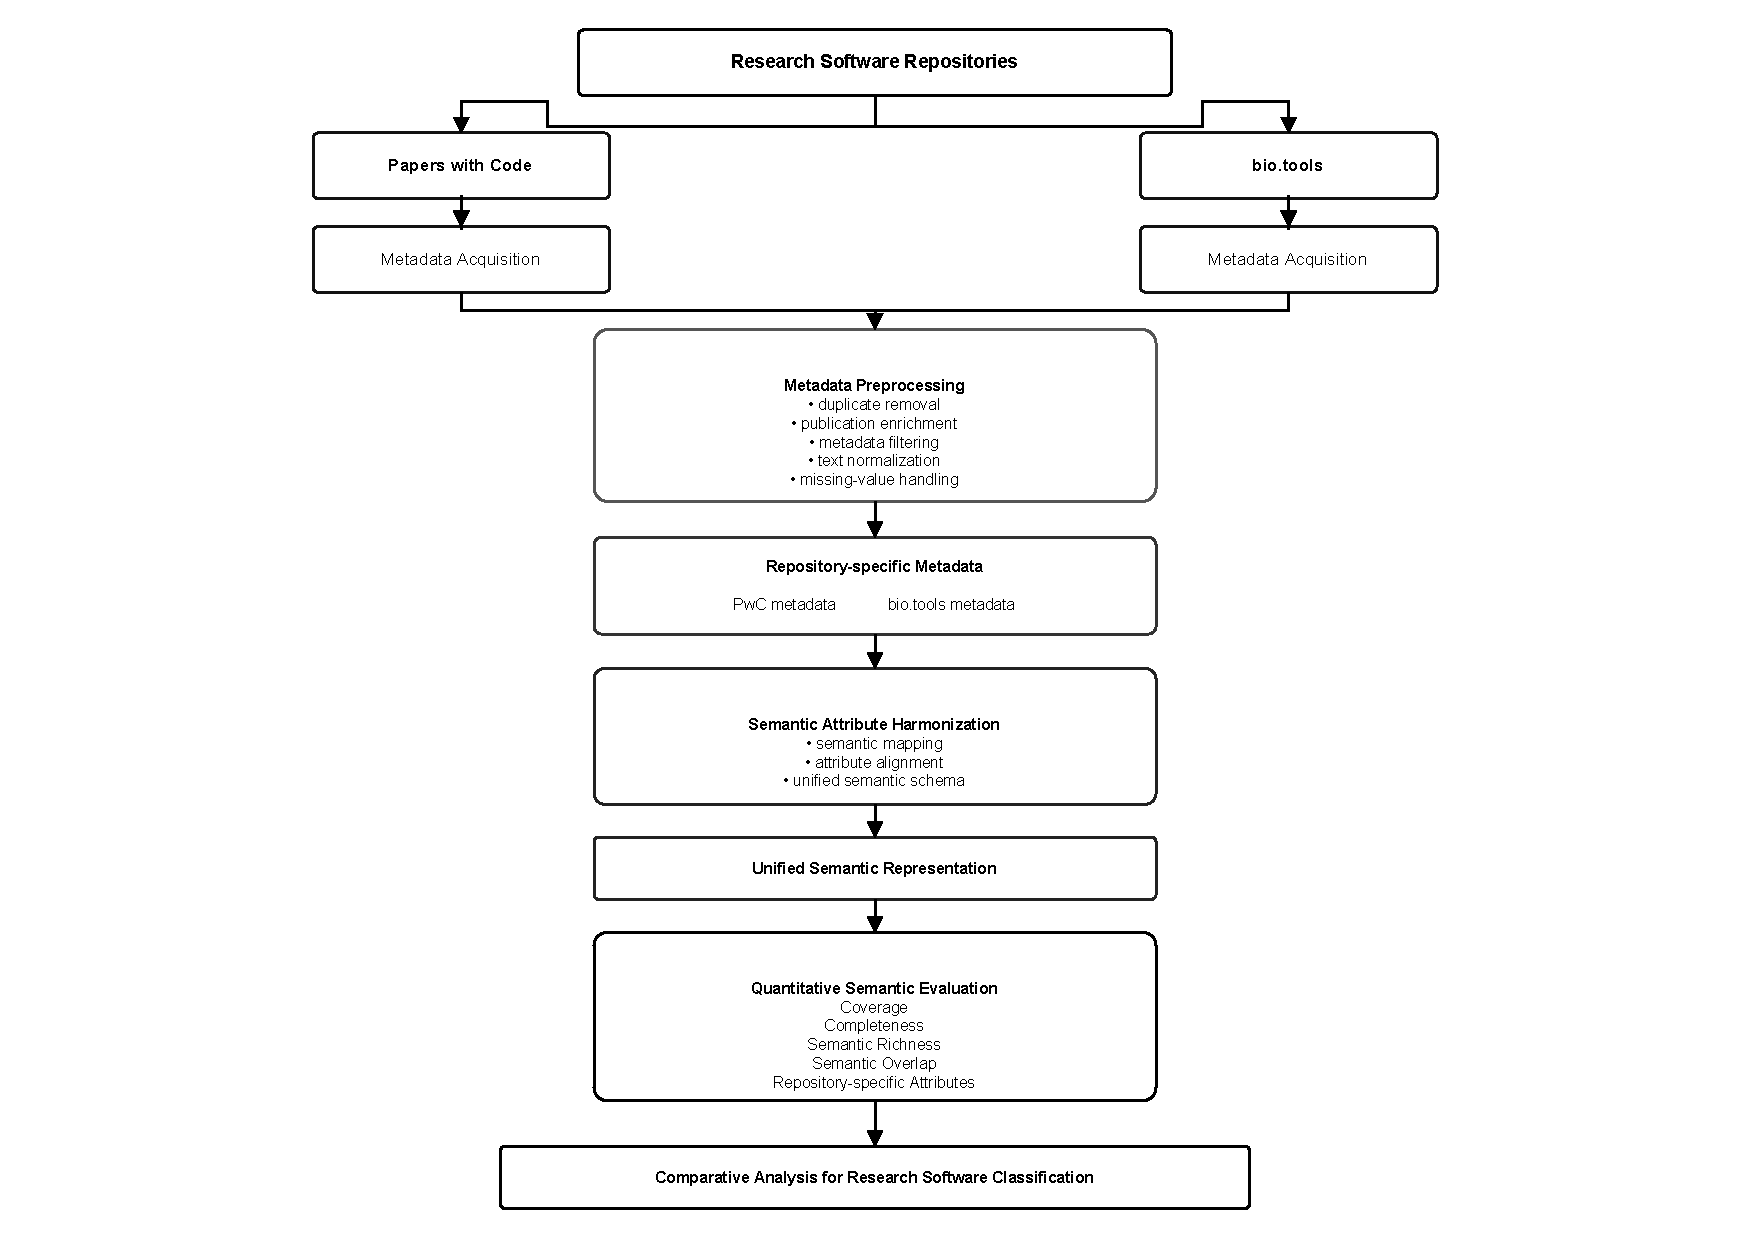
\includegraphics[width=\textwidth]{figures/methodology_pipeline.pdf}
\caption{Methodology pipeline for semantic metadata harmonization and quantitative evaluation.}
\label{fig:methodology-pipeline}
\end{figure}

\subsection{Preprocessing and Missing Values}
\label{subsec:methodology-preprocessing}

Records were normalized using the repository implementation. Text fields were whitespace-normalized and null-like strings such as \texttt{nan}, \texttt{none}, and \texttt{null} were treated as missing. List-valued fields were parsed, deduplicated, and counted as populated only when at least one usable normalized value remained. Papers with Code duplicates were handled using normalized publication titles before repository association. bio.tools records were aligned from tool metadata and publication metadata; multiple DOI-linked publications could create multiple software-publication records before final filtering.

\subsection{Unified Semantic Framework}
\label{subsec:semantic-framework}

The final retained fields were mapped to semantic dimensions using their conceptual meaning. A semantic dimension was considered populated when at least one mapped final-dataset field contained a usable value. Table~\ref{tab:semantic-crosswalk} shows the mapping used in the manuscript. Dimensions not retained as structured fields in the final dataset are shown explicitly rather than inferred from source-level metadata that is not present in the final package.

\begin{table}[htbp]
\centering
\small
\caption{Semantic-dimension mapping used for the final dataset package.}
\label{tab:semantic-crosswalk}
\begin{tabularx}{\textwidth}{p{3.4cm}XX}
\toprule
Semantic Dimension & Papers with Code fields & bio.tools fields \\
\midrule
Software Identifier & \texttt{item\_id} & \texttt{item\_id} \\
Software Name & \texttt{software\_name}, \texttt{repository\_title} & \texttt{software\_name}, \texttt{repository\_title} \\
Software Description & \texttt{software\_description}, \texttt{repository\_description}, \texttt{somef\_description} & \texttt{software\_description}, \texttt{repository\_description}, \texttt{somef\_description} \\
Publication Metadata & \texttt{paper\_title}, \texttt{paper\_abstract}, \texttt{publication\_url} & \texttt{paper\_title}, \texttt{paper\_abstract}, \texttt{publication\_url} \\
Research Domain & \texttt{labels} & \texttt{labels} \\
Software Functionality & \texttt{tasks}, \texttt{methods}, \texttt{secondary\_labels} & \texttt{tasks}, \texttt{methods}, \texttt{secondary\_labels} \\
Source Code Repository & \texttt{repository\_url} & \texttt{repository\_url} \\
Documentation & \texttt{readme\_content} & \texttt{readme\_content} \\
Input/Output Data, Data Format, Programming Language, License, Benchmarks, Evaluation Metrics & Not represented in \texttt{final\_combined.jsonl} & Not represented in \texttt{final\_combined.jsonl} \\
\bottomrule
\end{tabularx}
\end{table}

\subsection{Semantic Metadata Metrics}
\label{subsec:semantic-metrics}

For semantic dimension \(a\) and source \(s\), metadata coverage was computed as
\[
\mathrm{coverage}(a,s)=\frac{\left|\{r \in R_s : a \text{ has a usable value in } r\}\right|}{|R_s|}.
\]
When a dimension was represented by multiple fields, a record was counted once if any mapped field was populated.

Completeness was computed per record using the source-specific applicable final fields:
\[
C_r=\frac{\sum_{f \in A_s} I(r,f)}{|A_s|},
\]
where \(A_s\) is the set of applicable descriptive semantic fields for source \(s\), and \(I(r,f)=1\) when field \(f\) is usable after normalization. Semantic richness was summarized by the number of final labels, populated semantic fields, and unique controlled semantic values per record. Semantic overlap was computed at literal label, schema, and field-availability levels using the Jaccard coefficient.

\subsection{Classification Methodology}
\label{subsec:classification-methodology}

The completed classification experiments use the final labelled datasets and a deterministic 80/20 train/test split with random seed 42. Single-label tasks predict exactly one label per record and use stratification when label support permits. Multi-label tasks binarize the label set and evaluate one-vs-rest predictions. The completed full comparison in the repository uses TF--IDF unigram/bigram features and a balanced LinearSVC classifier. The TF--IDF vectorizer uses a maximum of 50,000 features, n-grams of length one and two, and \(\mathrm{min\_df}=2\) in the completed full-dataset training output. The classifier uses class weighting and random seed 42.

The evaluated attribute sets are abstract only, title only, repository title/keywords, abstract plus README/description, abstract plus repository title/keywords, all publication metadata, all repository metadata, and all available metadata. The attribute-set definitions used for the completed results follow the saved run configuration in \texttt{results/training/run\_configuration.json}, which excludes target label fields from the predictor text. The planned keyword-only setting is not reported in the completed table because repository keyword coverage is zero in the final dataset package.

For single-label classification, the manuscript reports accuracy and macro-, micro-, and weighted-F1. For multi-label classification, it reports macro-, micro-, and weighted-F1 together with subset accuracy. Precision, recall, and F1 are defined in the usual way:
\[
P=\frac{TP}{TP+FP}, \quad R=\frac{TP}{TP+FN}, \quad F_1=\frac{2PR}{P+R}.
\]
Macro-F1 averages per-label F1 scores equally, micro-F1 pools decisions across labels, and weighted-F1 weights labels by support.

Neural embedding, fine-tuned transformer, and LLM prompting pipelines are implemented or documented in the repository, but they are not completed in the verified full classification table used here. They are therefore not reported as completed results.

\section{Semantic Metadata Analysis}
\label{sec:semantic-analysis}

\subsection{Metadata Coverage}
\label{subsec:semantic-coverage}

Table~\ref{tab:semantic-dimension-coverage} reports semantic-dimension coverage by source.

\begin{table}[htbp]
\centering
\small
\caption{Metadata coverage by unified semantic dimension and source.}
\label{tab:semantic-dimension-coverage}
\begin{tabular}{llll}
\toprule
Semantic Dimension & PwC Coverage & bio.tools Coverage & Availability \\
\midrule
Software Identifier & 42,669 / 42,669 (100.00\%) & 14,150 / 14,150 (100.00\%) & Shared \\
Software Name & 42,669 / 42,669 (100.00\%) & 14,150 / 14,150 (100.00\%) & Shared \\
Software Description & 36,032 / 42,669 (84.45\%) & 14,150 / 14,150 (100.00\%) & Shared \\
Publication Metadata & 42,669 / 42,669 (100.00\%) & 14,150 / 14,150 (100.00\%) & Shared \\
Research Domain & 42,669 / 42,669 (100.00\%) & 14,150 / 14,150 (100.00\%) & Shared \\
Software Functionality & 42,669 / 42,669 (100.00\%) & 13,521 / 14,150 (95.55\%) & Shared \\
Input / Output Data & 0 / 42,669 (0.00\%) & 0 / 14,150 (0.00\%) & Not represented \\
Data Format & 0 / 42,669 (0.00\%) & 0 / 14,150 (0.00\%) & Not represented \\
Programming Language & 0 / 42,669 (0.00\%) & 0 / 14,150 (0.00\%) & Not represented \\
License & 0 / 42,669 (0.00\%) & 0 / 14,150 (0.00\%) & Not represented \\
Source Code Repository & 42,669 / 42,669 (100.00\%) & 14,150 / 14,150 (100.00\%) & Shared \\
Documentation & 41,405 / 42,669 (97.04\%) & 13,488 / 14,150 (95.32\%) & Shared \\
Benchmarks & 0 / 42,669 (0.00\%) & 0 / 14,150 (0.00\%) & Not represented \\
Evaluation Metrics & 0 / 42,669 (0.00\%) & 0 / 14,150 (0.00\%) & Not represented \\
\bottomrule
\end{tabular}
\end{table}

Eight of the fourteen evaluated dimensions are represented above the 5\% availability threshold in both repositories. Software identifiers, software names, publication metadata, research-domain labels, and source-code repository links are complete in the final datasets. Documentation is also highly available, with README content for 97.04\% of Papers with Code records and 95.32\% of bio.tools records. Six dimensions are not represented as structured fields in the final combined dataset: input/output data, data format, programming language, license, benchmarks, and evaluation metrics. This means they cannot be evaluated from the final package, not that the original repositories necessarily lack such information.

\subsection{Metadata Completeness}
\label{subsec:semantic-completeness}

\begin{table}[htbp]
\centering
\small
\caption{Descriptive statistics for metadata completeness by source.}
\label{tab:semantic-completeness-descriptive-statistics}
\begin{tabular}{lrrrrr}
\toprule
Source & Mean & Median & Standard Deviation & Minimum & Maximum \\
\midrule
Papers with Code & 0.8089 & 0.8333 & 0.0460 & 0.5833 & 0.8333 \\
bio.tools & 0.8192 & 0.8462 & 0.0550 & 0.4615 & 0.8462 \\
\bottomrule
\end{tabular}
\end{table}

Both repositories have high completeness under the implemented metric. Papers with Code has mean completeness 0.8089 and median 0.8333. bio.tools has mean completeness 0.8192 and median 0.8462. The maximum values are below one because completeness is computed over the applicable final fields, including fields that are systematically absent or below coverage threshold in the retained package.

\subsection{Semantic Richness}
\label{subsec:semantic-richness}

\begin{table}[htbp]
\centering
\scriptsize
\caption{Descriptive statistics for semantic richness by repository.}
\label{tab:semantic-richness-descriptive-statistics}
\setlength{\tabcolsep}{3pt}
\begin{tabular}{lrrrrrrrrr}
\toprule
Repository & Mean Labels & Median Labels & SD Labels & Mean Populated Dimensions & Median Populated Dimensions & SD Populated Dimensions & Mean Unique Semantic Values & Median Unique Semantic Values & SD Unique Semantic Values \\
\midrule
Papers with Code & 1.1405 & 1.0000 & 0.3736 & 9.7063 & 10.0000 & 0.5520 & 15.3426 & 9.0000 & 12.5680 \\
bio.tools & 2.1522 & 2.0000 & 0.8598 & 10.6490 & 11.0000 & 0.7149 & 4.8049 & 5.0000 & 1.7290 \\
\bottomrule
\end{tabular}
\end{table}

bio.tools records have more labels per record on average, with mean 2.1522 compared with 1.1405 for Papers with Code. bio.tools also has a slightly higher mean number of populated semantic fields. Papers with Code, however, has a larger mean number of unique controlled semantic values per record, 15.3426 compared with 4.8049 for bio.tools, and much higher variability.

\subsection{Semantic Overlap}
\label{subsec:semantic-overlap}

\begin{table}[htbp]
\centering
\small
\caption{Semantic overlap between Papers with Code and bio.tools.}
\label{tab:semantic-overlap-summary}
\begin{tabular}{lrrrrr}
\toprule
Overlap Level & PwC Count & bio.tools Count & Shared & Union & Jaccard \\
\midrule
Literal final label strings & 6 & 12 & 0 & 18 & 0.0000 \\
Shared applicable schema fields & 12 & 13 & 11 & 14 & 0.7857 \\
Field availability at 5\% threshold & 10 & 11 & 9 & 12 & 0.7500 \\
\bottomrule
\end{tabular}
\end{table}

The final label vocabularies have no literal string overlap. This result reflects different domain vocabularies and curation schemes rather than a demonstrated absence of conceptual similarity. At the schema level, eleven of fourteen applicable fields overlap. At the availability level, nine of twelve available fields are shared.

\subsection{Repository-specific Field Availability}
\label{subsec:repository-specific-availability}

\begin{table}[htbp]
\centering
\small
\caption{Repository-specific field availability using the 5\% coverage threshold.}
\label{tab:repository-specific-attribute-availability}
\begin{tabularx}{\textwidth}{p{3.2cm}X}
\toprule
Availability Class & Final-dataset Fields \\
\midrule
Shared & \texttt{paper\_title}, \texttt{paper\_abstract}, \texttt{publication\_url}, \texttt{repository\_url}, \texttt{repository\_title}, \texttt{readme\_content}, \texttt{somef\_description}, \texttt{tasks}, \texttt{secondary\_labels} \\
Papers with Code only & \texttt{methods} \\
bio.tools only & \texttt{software\_name}, \texttt{software\_description} \\
Below threshold in both & \texttt{repository\_description}, \texttt{repository\_keywords} \\
\bottomrule
\end{tabularx}
\end{table}

The field-level availability analysis complements the dimension-level coverage table. Some conceptual dimensions are shared because they are represented by alternative fields, even when an individual field is source-specific. For example, the software-name dimension is shared at the dimension level because repository titles are available for both sources, while the dedicated \texttt{software\_name} field is populated only for bio.tools.

\section{Research Software Classification Experiments and Results}
\label{sec:classification-results}

\subsection{Experimental Overview}
\label{subsec:classification-overview}

The completed classification results used in this manuscript are the local TF--IDF LinearSVC experiments over four final datasets. Table~\ref{tab:classification-datasets} summarizes the datasets and splits.

\begin{table}[htbp]
\centering
\small
\caption{Classification datasets used in the completed TF--IDF LinearSVC experiments.}
\label{tab:classification-datasets}
\begin{tabular}{lrrrr}
\toprule
Dataset & Records & Train & Test & Labels \\
\midrule
PwC single-label & 37,058 & 29,646 & 7,412 & 6 \\
PwC multi-label & 42,669 & 34,135 & 8,534 & 6 \\
bio.tools single-label & 3,272 & 2,617 & 655 & 11 \\
bio.tools multi-label & 14,150 & 11,320 & 2,830 & 12 \\
\bottomrule
\end{tabular}
\end{table}

\TODO{Run and report the disabled SBERT or frozen-transformer, fine-tuned transformer, and OpenAI prompting experiments before making claims about neural or LLM-based classifiers. The verified full classification table used here contains only TF--IDF LinearSVC experiments.}

\subsection{Best-performing Completed Configurations}
\label{subsec:classification-best}

Table~\ref{tab:classification-best-results} reports the best completed configuration for each dataset, selected by macro-F1.

\begin{table}[htbp]
\centering
\small
\caption{Best completed classification result for each dataset, selected by macro-F1.}
\label{tab:classification-best-results}
\begin{tabular}{llrrrr}
\toprule
Dataset & Attribute Set & Macro-F1 & Micro-F1 & Weighted-F1 & Accuracy/Sub.Acc. \\
\midrule
PwC single-label & All available metadata & 0.8671 & 0.9575 & 0.9573 & 0.9575 \\
PwC multi-label & All available metadata & 0.8782 & 0.9407 & 0.9408 & 0.8859 \\
bio.tools single-label & All available metadata & 0.4728 & 0.9191 & 0.9093 & 0.9191 \\
bio.tools multi-label & All available metadata & 0.6644 & 0.8671 & 0.8614 & 0.5859 \\
\bottomrule
\end{tabular}
\end{table}

All four datasets achieve their best macro-F1 with the all-available-metadata attribute set. Papers with Code performs substantially better than bio.tools under this completed classifier. The best Papers with Code macro-F1 values are 0.8671 for the single-label setting and 0.8782 for the multi-label setting. The corresponding bio.tools values are 0.4728 and 0.6644.

\subsection{Comparison of Metadata Attributes}
\label{subsec:classification-attributes}

Table~\ref{tab:classification-attribute-comparison} compares macro-F1 across metadata attribute sets.

\begin{table}[htbp]
\centering
\scriptsize
\caption{Macro-F1 of completed TF--IDF LinearSVC experiments by dataset and metadata attribute set.}
\label{tab:classification-attribute-comparison}
\setlength{\tabcolsep}{3pt}
\begin{tabular}{lrrrr}
\toprule
Attribute Set & PwC Single & PwC Multi & bio.tools Single & bio.tools Multi \\
\midrule
Abstract & 0.7665 & 0.7613 & 0.3000 & 0.5058 \\
Title & 0.5518 & 0.5543 & 0.3239 & 0.4392 \\
Repository title/keywords & 0.2754 & 0.2495 & 0.2164 & 0.2175 \\
Abstract + README/description & 0.6605 & 0.7027 & 0.4165 & 0.5472 \\
Abstract + repository title/keywords & 0.7659 & 0.7593 & 0.3199 & 0.5127 \\
Publication metadata & 0.7875 & 0.7813 & 0.3101 & 0.5346 \\
Repository metadata & 0.5252 & 0.5552 & 0.3904 & 0.4590 \\
All available metadata & 0.8671 & 0.8782 & 0.4728 & 0.6644 \\
\bottomrule
\end{tabular}
\end{table}

Publication metadata outperforms titles alone in all four settings, and all available metadata gives the strongest macro-F1 in all four settings. Repository-title/keyword representations are consistently weakest, which is consistent with the final package having zero usable repository-keyword coverage. Adding README and description fields improves bio.tools macro-F1 relative to abstracts alone, while the strongest results still require combining all retained fields.

\section{Discussion}
\label{sec:discussion}

\subsection{Answering the Research Questions}
\label{subsec:discussion-rqs}

RQ1 asked which attributes are represented and how they can be organized. The final retained package supports a unified framework covering identifiers, names, descriptions, publication metadata, research domains, functionality, repository links, and documentation. It does not retain structured input/output data, data formats, programming languages, licenses, benchmarks, or evaluation metrics.

RQ2 asked how the repositories overlap. Literal label overlap is zero, but schema-level overlap is substantial, with a Jaccard coefficient of 0.7857. Field availability overlap is also high, with a Jaccard coefficient of 0.7500. The absence of literal label overlap should not be interpreted as evidence that the repositories describe fundamentally different types of Research Software. Rather, it reflects the use of distinct domain-specific vocabularies and metadata schemas. This finding reinforces the need for semantic harmonization, demonstrating that interoperability between heterogeneous Research Software repositories is achieved through conceptual alignment rather than direct vocabulary matching.

RQ3 asked how the repositories differ in coverage, completeness, richness, and repository-specific attributes. Both have high completeness, but their richness profiles differ. bio.tools has more labels per record and slightly more populated fields, while Papers with Code has more unique controlled semantic values and greater variability. Dedicated software-name and software-description fields are bio.tools-specific at the field level, while methods are Papers with Code-specific.

RQ4 asked how metadata attributes support classification. In the completed TF--IDF LinearSVC experiments, all available metadata is the strongest attribute set for all datasets. Publication metadata is consistently stronger than title-only metadata, while repository-title/keyword metadata performs poorly.

RQ5 asked how results differ by label setting and repository. Papers with Code performs better than bio.tools in both single-label and multi-label settings. bio.tools has more labels and a more domain-specific ontology-derived label space, and its macro-F1 values remain lower despite high micro-F1 and weighted-F1 in some settings.

\subsection{Implications for Research Software Classification}
\label{subsec:discussion-classification}

The classification results suggest that attribute coverage alone is not sufficient to predict performance. Titles and repository links have complete or near-complete coverage, but title-only and repository-title/keyword representations are not the best predictors. The strongest results come from combining publication metadata, repository-derived documentation, SoMEF descriptions, tasks, methods, and secondary labels. This indicates that predictive metadata value depends on both availability and semantic specificity.

README-derived and description-derived fields are useful, particularly when combined with abstracts, but they do not replace publication metadata. Publication metadata remains important because titles and abstracts often encode research domain and methodological context. For cross-repository classifiers, the results suggest that harmonized field groups are more promising than direct label-vocabulary matching.

\subsection{Implications for Metadata Standards and Repositories}
\label{subsec:discussion-standards}

The final retained package lacks structured programming language, license, data-format, benchmark, and evaluation-metric fields. These dimensions are relevant to standards such as CodeMeta, CFF, EDAM, and software registry schemas, but they cannot be analysed unless extraction pipelines preserve them in the final analysis package. Repositories and harmonization workflows should therefore retain structured source-level fields, provenance, and controlled identifiers alongside textual descriptions.

\subsection{Implications for Knowledge Graphs and Interoperability}
\label{subsec:discussion-kg}

The semantic-overlap results support a knowledge-graph view of interoperability. Direct vocabulary matching is insufficient, but schema-level and concept-level alignment can reveal shared structure. Future integrations should preserve provenance for each mapped field and should support explicit ontology alignment between Papers with Code concepts and EDAM categories. Ontology matching methods provide a possible direction for this future work \cite{Euzenat2013OntologyMatching,Otero2015OntologyMatching,Trojahn2022Foundational}.

\section{Threats to Validity}
\label{sec:threats}

\subsection{Dataset and Selection Validity}
\label{subsec:threats-dataset}

The final datasets include only records retained by the implemented pipeline. Filtering by GitHub repository URL excludes software without GitHub links. bio.tools records are affected by publication expansion and EDAM top-level mapping, and some records are excluded when labels cannot be mapped. The repositories also represent different domains: Papers with Code is concentrated in artificial intelligence, whereas bio.tools covers Life Science software. These domain differences limit direct source-to-source interpretation.

\subsection{Construct Validity}
\label{subsec:threats-construct}

Completeness and richness are operational definitions over retained final fields, not universal measures of metadata quality. The 5\% availability threshold is a pragmatic cutoff and may hide rare but meaningful metadata. Literal label overlap underestimates conceptual similarity because no ontology-based alignment between Papers with Code labels and EDAM labels is implemented.

\subsection{Internal Validity}
\label{subsec:threats-internal}

Preprocessing choices influence the final representation. Title-based duplicate handling, text normalization, missing-value treatment, and enrichment quality may affect coverage and classification. The completed classification experiments use a single deterministic train/test split rather than cross-validation. The same split is reused across attribute sets, which supports paired comparison within a dataset, but robustness across alternative splits remains untested.

\subsection{External Validity}
\label{subsec:threats-external}

The study covers two repositories and should not be generalized without caution to other Research Software registries, package indexes, institutional catalogs, or archival infrastructures. It is also centered on GitHub-linked software. Results may differ for software hosted elsewhere, for software without publications, or for repositories with stronger structured metadata requirements.

\subsection{Reproducibility}
\label{subsec:threats-reproducibility}

The analyses are grounded in repository scripts and generated output files, and the implemented train/test experiments use random seed 42. However, some provenance details, such as exact external snapshot dates for every raw source, are not fully represented in the final manuscript evidence base. The neural, fine-tuned transformer, and LLM classification pipelines remain unreported until completed outputs are generated and validated.

\section{Conclusion}
\label{sec:conclusion}

This paper compared semantic metadata attributes from Papers with Code and bio.tools and evaluated their usefulness for Research Software classification. The final harmonized dataset contains 56,819 labelled records, with 42,669 from Papers with Code and 14,150 from bio.tools. The semantic analysis shows no literal overlap between final label vocabularies, but substantial overlap at schema and field-availability levels. Metadata completeness is high in both repositories, while semantic richness differs: bio.tools has more labels and populated fields per record, whereas Papers with Code has more unique controlled semantic values.

The completed classification experiments show that all available metadata gives the strongest macro-F1 for each evaluated dataset under TF--IDF LinearSVC. Papers with Code is more readily classified than bio.tools, while bio.tools remains more difficult under macro-F1 because of its label space and imbalance. These findings indicate that semantic harmonization and classification evaluation are complementary: harmonization reveals conceptual alignment across repositories, while classification exposes which retained attributes are practically predictive.

Future work should complete the disabled neural, transformer, and LLM pipelines; add ontology alignment between Papers with Code and EDAM; evaluate additional Research Software repositories; preserve currently unrepresented fields such as programming language, license, data format, benchmark, and evaluation metadata; and study cross-domain transfer and improved multi-label classification.

\backmatter

\bmhead{Supplementary information}
The analysis scripts, generated tables, and final dataset package are retained in the project repository. Missing-result placeholders in this manuscript refer to implemented but not completed classification pipelines.

\bmhead{Acknowledgements}
Acknowledgements will be added in the final submission version.

\section*{Declarations}

\bmhead{Funding}
Funding information is not provided in the current repository version.

\bmhead{Competing interests}
The authors declare no competing interests.

\bmhead{Data availability}
The manuscript analyses the local final dataset package and generated result files retained in the project repository.

\bmhead{Code availability}
The preprocessing, semantic-analysis, and classification scripts are retained in the project repository.

\bibliography{sn-bibliography}

\end{document}
